\section[Correction to $dN/dn_\textrm{sel}$]{Correction to $\mathbf{dN/dn_\textrm{sel}}$}\label{section:star_dNdnch}
In order to express the multiplicity distribution in terms of the number of charged particles, $n_\textrm{ch}$, instead of the number of selected tracks, $n_\textrm{sel}$.%,  the observed $n_\textrm{sel}$ distribution was corrected for detector effects after subtraction of accidental and non-SD backgrounds. 
The  following procedure based on the Bayesian unfolding~\cite{unfolding:2016mok,unfolding:DAgostini} was used. First, the~$n_\textrm{sel}$ distribution was corrected for vertex reconstruction effects by applying event-by-event weights, $w_\textrm{ev}^\textrm{vrt}(n_\textrm{vrt}^\textrm{global},|\Delta z_0|)$. The number of events in which $n_\textrm{ch}$ are produced, $N_\textrm{ev}(n_\textrm{ch})$, can be associated with the number of events in which $n_\textrm{sel}$ are reconstructed, $N_\textrm{ev}(n_\textrm{sel})$.
\begin{comment}
\begin{equation}
N_\textrm{ev}\left(n_\textrm{ch}|n_\textrm{sel}\right)=N_\textrm{ev}\left(n_\textrm{sel}\right)\cdot P\left(n_\textrm{ch}|n_\textrm{sel}\right)
\end{equation}
where $P(n_\textrm{ch}|n_\textrm{sel})$ is the conditional probability of having $n_\textrm{ch}$ charged particles in an event in which  $n_\textrm{sel}$ tracks were found.
\end{comment}
Since there are several possible $n_\textrm{sel}$ observed in  $n_\textrm{ch}$ event,  $N_\textrm{ev}(n_\textrm{ch})$ is given by:
\begin{equation}
\begin{array}{ccccc}
N_\textrm{ev}(n_\textrm{ch})&=&&\displaystyle\sum_{n_\textrm{sel}=0}P(n_\textrm{ch}|n_\textrm{sel})\cdot N_\textrm{ev}(n_\textrm{sel})\\
&=&\frac{1}{\epsilon_{m}(n_\textrm{ch})\epsilon_{r}(n_\textrm{ch})}&\displaystyle\sum_{n_\textrm{sel}=2}^{8}P(n_\textrm{ch}|n_\textrm{sel})\cdot N_\textrm{ev}(n_\textrm{sel})
\end{array}
\end{equation}
where:
\begin{description}
	\item $P(n_\textrm{ch}|n_\textrm{sel})$ is the conditional probability of having $n_\textrm{ch}$ charged particles in an event in which  $n_\textrm{sel}$ tracks were found,
	\item $\epsilon_{m}(n_\textrm{ch})$ is a factor, which recovers events that are lost due to TPC track reconstuction and  TOF matching inefficiencies, i.e. those with $n_\textrm{ch}\geq2$ but $n_\textrm{sel}<2$,
	\item $\epsilon_{r}(n_\textrm{ch})$ is a factor, which recovers  events which are lost due to fake tracks, i.e. those with $n_\textrm{ch}\leq 8$ but $n_\textrm{sel}> 8$. It was checked that this effect is negligible (smaller than $1\permil$) and can be omitted. 
\end{description}
Figure~\ref{fig:correctionSTAR} shows $\epsilon_{m}(n_\textrm{ch})$  in three ranges of $\xi$. It was derived from MC and varies from about $25\%$ for $n_\textrm{ch}=2$ to $95\%$ for $n_\textrm{ch}=8$. Since there are additional data-driven corrections to \ac{TPC} and TOF efficiences,  MC simulations were modified by randomly removing or adding tracks. This was done in accordance with differences in the~efficiencies between data and MC. 
Figure~\ref{fig:correctionSTAR_syst} shows  $\epsilon_{m}(n_\textrm{ch})$ calculated in three ranges of $\xi$ using no-pile-up PYTHIA~8 and EPOS SD+SD$^\prime$. The~differences between
these two models, which are up to $8\%$ for $n_\textrm{ch}=2$ and $0.1<\xi<0.2$, were symmetrized and taken as a~systematic uncertainty.


\begin{figure}[h!]
	\centering
		\begin{subfigure}{.49\textwidth}
			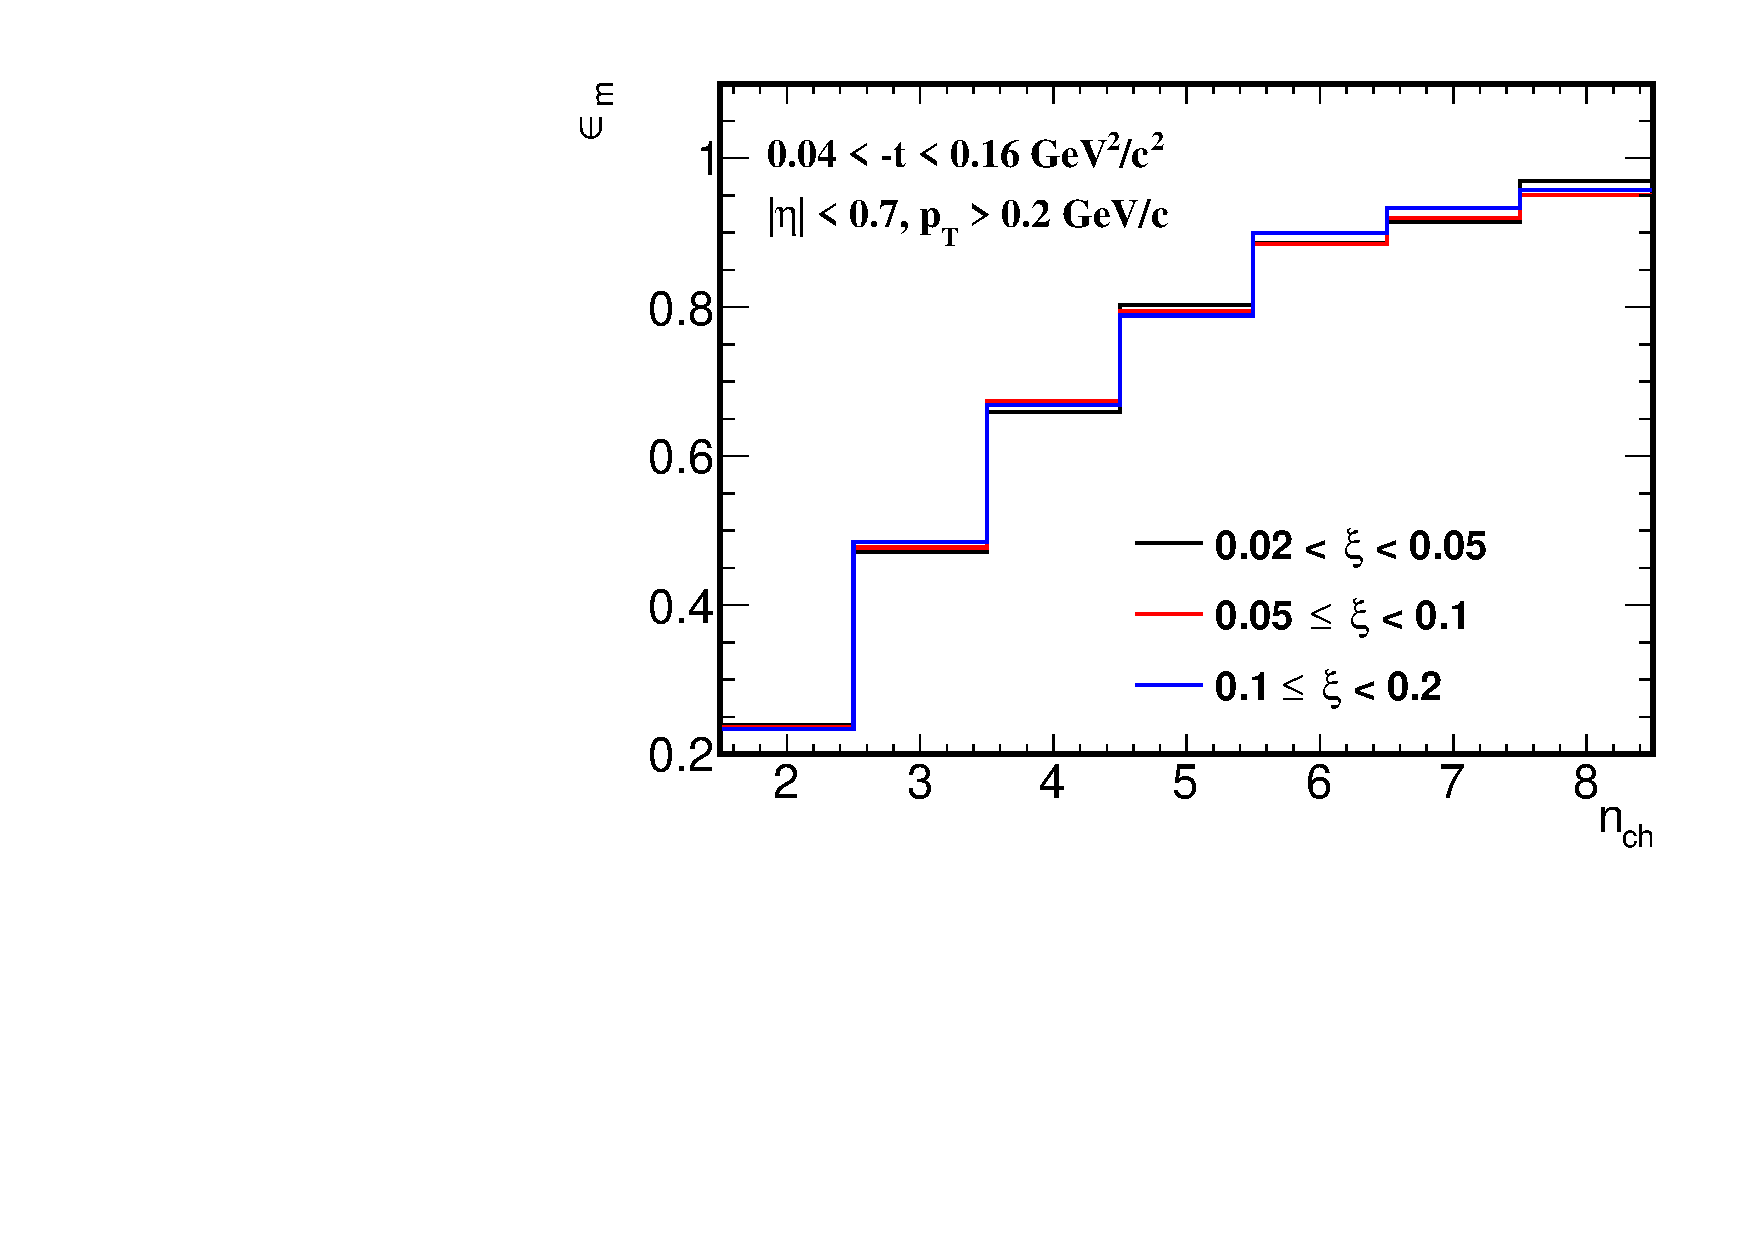
\includegraphics[width=\textwidth,page=1]{chapters/chrgSTAR/img/unfolding/correction_0.pdf}
		\end{subfigure}
		\begin{minipage}{.49\textwidth}
			\caption{$\epsilon_{m}(n_\textrm{ch})$  calculated separately in three ranges of $\xi$ using PYTHIA~8 embedding MC.}
			\label{fig:correctionSTAR}
		\end{minipage}
	
\end{figure}


\begin{figure}[h!]
	\centering
	\begin{subfigure}{.47\textwidth}
		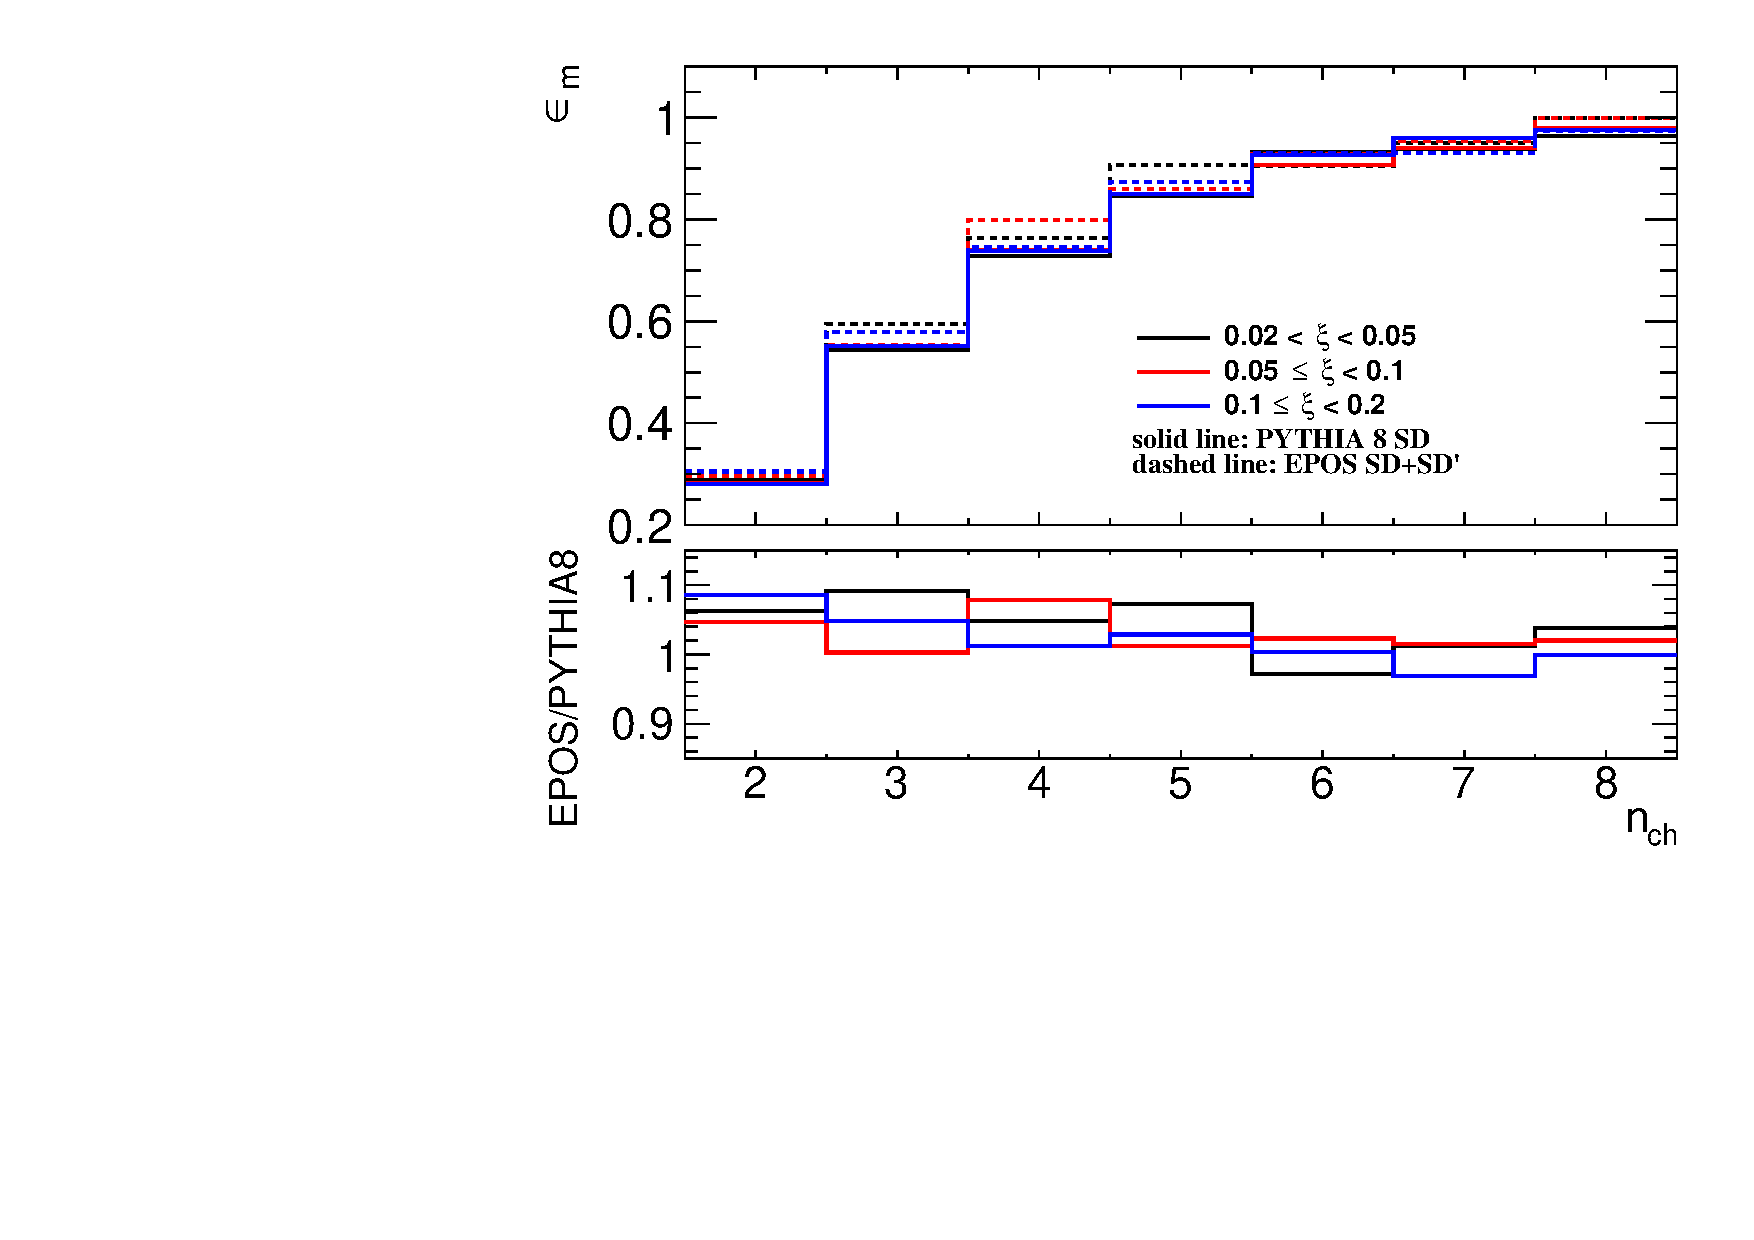
\includegraphics[width=\textwidth,page=1]{chapters/chrgSTAR/img/unfolding/nch_m2_nsel_s2.pdf}
	\end{subfigure}
	\begin{minipage}{.48\textwidth}
		\caption{Comparison of $\epsilon_{m}(n_\textrm{ch})$  calculated separately in three ranges of $\xi$ using PYTHIA~8 SD and EPOS SD+SD$^\prime$ no-pile-up MCs.}
		\label{fig:correctionSTAR_syst}
	\end{minipage}
	
\end{figure}

\noindent The  probability $P(n_\textrm{ch}|n_\textrm{sel})$ can be derived using Bayes' theorem, which can be stated mathematically in terms of charged particle and charged track multiplicities as:
\begin{equation}
P\left(n_\textrm{ch}\right)\cdot P\left(n_\textrm{sel}|n_\textrm{ch}\right) = P\left(n_\textrm{ch}|n_\textrm{sel}\right)\cdot P\left(n_\textrm{sel}\right)
\end{equation}
where: $P(n_\textrm{sel})$ and $P(n_\textrm{ch})$ are probabilities of observing $n_\textrm{sel}$ and $n_\textrm{ch}$ respectivelly, $P(n_\textrm{ch}|n_\textrm{sel})$ and $P(n_\textrm{sel}|n_\textrm{ch})$ are conditional probabilities.
 
\noindent 
In order to improve the estimate of $P(n_\textrm{ch}|n_\textrm{sel})$, the~unfolding  is done iteratively:
\begin{itemize}
	\item In the~first iteration, it is assumed that: \\
	\begin{eqnarray}
	P(n_\textrm{ch}|n_\textrm{sel}) = P = P^{\textrm{MC}}(n_\textrm{sel}|n_\textrm{ch})\frac{P^\textrm{MC}(n_\textrm{ch})}{P^\textrm{MC}(n_\textrm{sel})}
	\end{eqnarray}
	\begin{equation}
	N_\textrm{ev}(n_\textrm{ch})=\frac{1}{\epsilon_{m}(n_\textrm{ch})}\sum_{n_\textrm{sel}=2}^{8}N_\textrm{ev}(n_\textrm{sel})\cdot P
	\end{equation}
	where $P^{\textrm{MC}}(n_\textrm{sel}|n_\textrm{ch})$, $P^\textrm{MC}(n_\textrm{ch})$ and $P^\textrm{MC}(n_\textrm{sel})$ are obtained from MC. $P^{\textrm{MC}}(n_\textrm{sel}|n_\textrm{ch})$ is the~same for each iteration.
	
	\item In the $(i+1)$th iteration we have:
	\begin{equation}
	P^{i+1}=P^{\textrm{MC}}(n_\textrm{sel}|n_\textrm{ch})\frac{N_\textrm{ev}^{i}(n_\textrm{ch})}{N_\textrm{ev}(n_\textrm{sel})}
	\end{equation}
	\begin{equation}
	N_\textrm{ev}^{i+1}(n_\textrm{ch})=\frac{1}{\epsilon_{m}(n_\textrm{ch})}\sum_{n_\textrm{sel}=2}^{8}N_\textrm{ev}(n_\textrm{sel})\cdot P^{i+1}
	\end{equation}
	where  $N_\textrm{ev}^i(n_\textrm{ch})$ is calculated in the previous iteration, and $N_\textrm{ev}(n_\textrm{sel})$ is taken from data.
\end{itemize}

The  unfolding matrices $P(n_\textrm{ch}|n_\textrm{sel})$  for each $\xi$ region, shown in Fig.~\ref{fig:responseSTAR}, were obtained from PYTHIA~8 embedding MC and used in all iterations of the above procedure. Similarly to $\epsilon_m(n_\textrm{ch})$, the~matrices were modified in order to take into account differences between data and PYTHIA~8. In order to  obtain statistically precise unfolding matrices,   all simulated events were used, i.e. also those with additional fake vertices (with $n_\textrm{sel}$ defined as a~number of primary tracks associated with the~best vertex).
The~systematic uncertainty related to limited statistics in PYTHIA~8 was estimated by performing $50$ pseudo-experiments, in which the~unfolding matrices were smeared according to their statistical uncertainties.
It affects mainly large charged-particle multiplicites, where it is about $8-10\%$, as shown in Fig.~\ref{fig:responseSTAR_uncert}.


\begin{figure}[h!]
	%\vspace{-0.5cm}
	\centering
	\begin{subfigure}{.49\textwidth}
		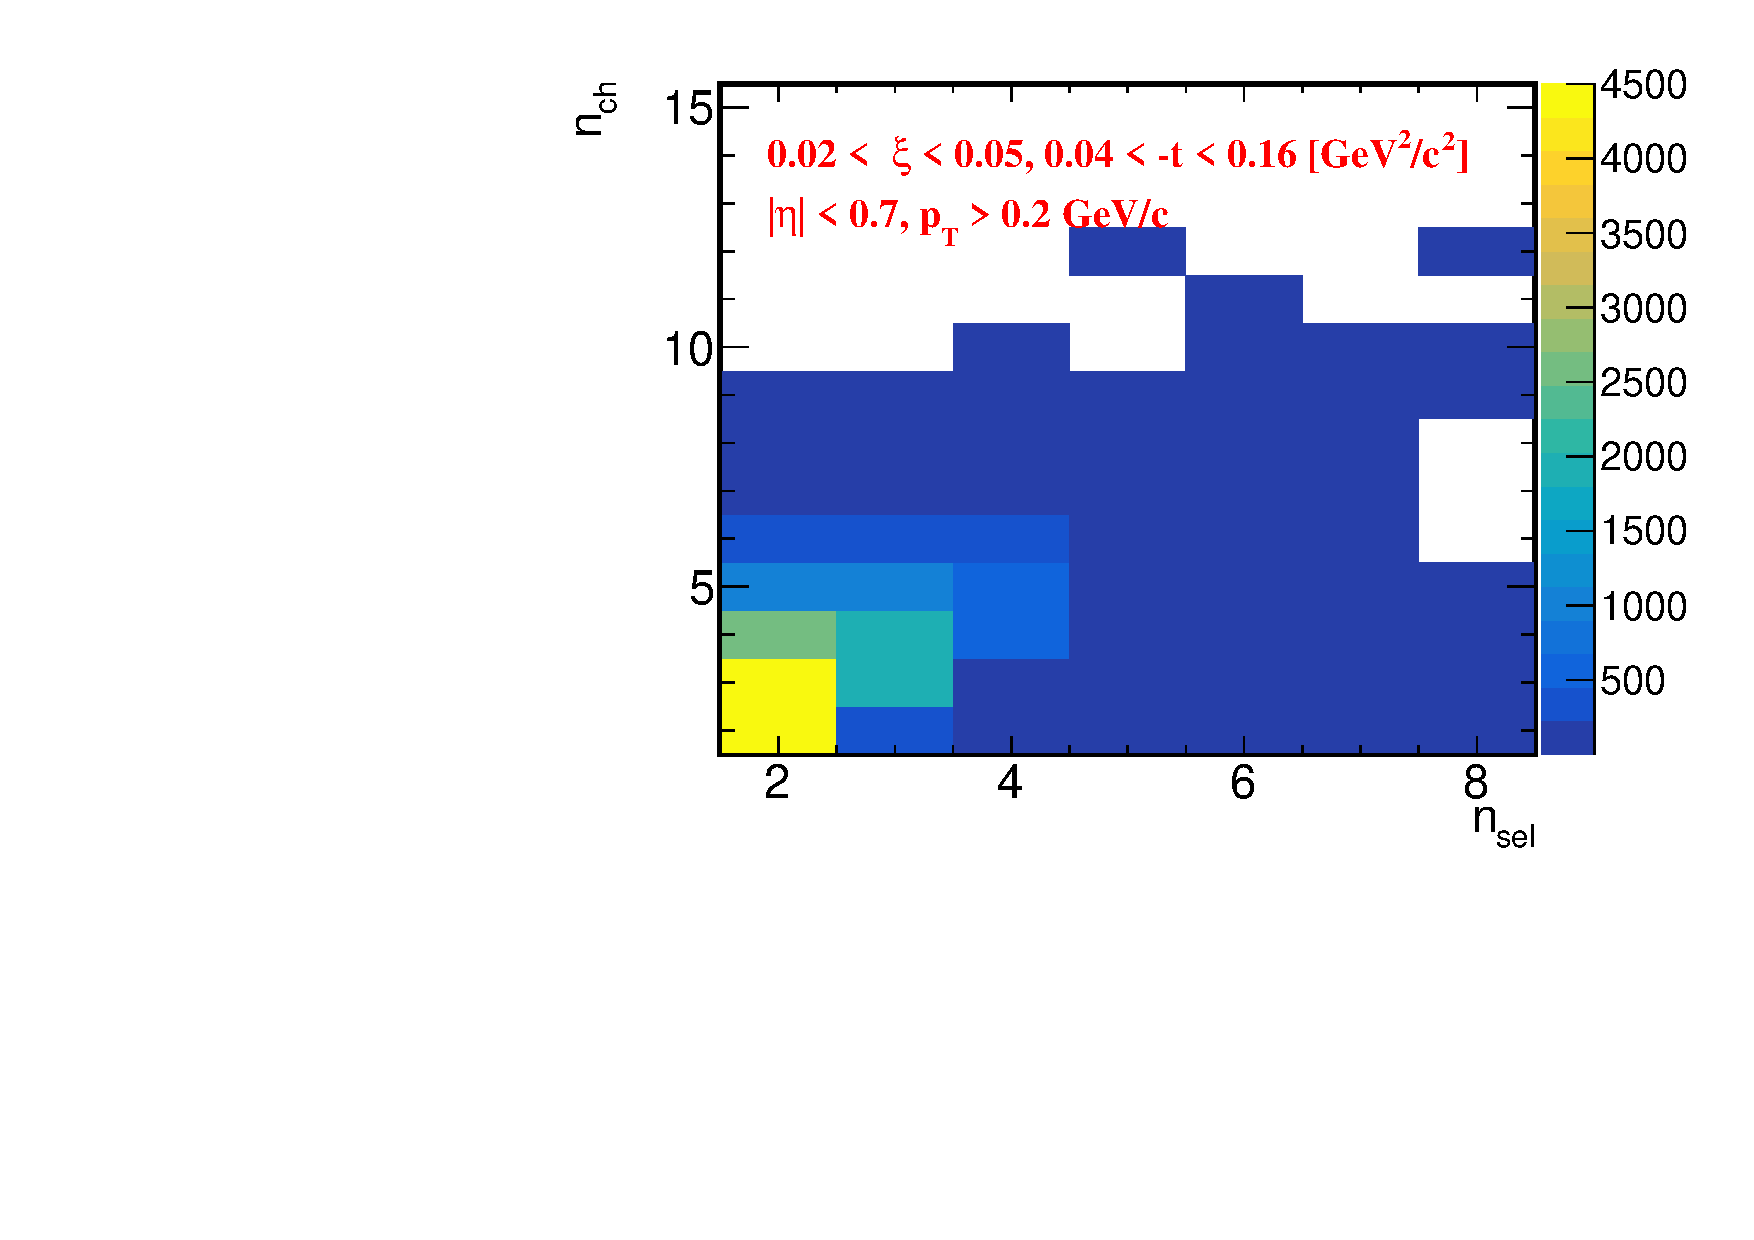
\includegraphics[width=\textwidth,page=1]{chapters/chrgSTAR/img/unfolding/matrix_0.pdf}
	\end{subfigure}
	\begin{subfigure}{.49\textwidth}
		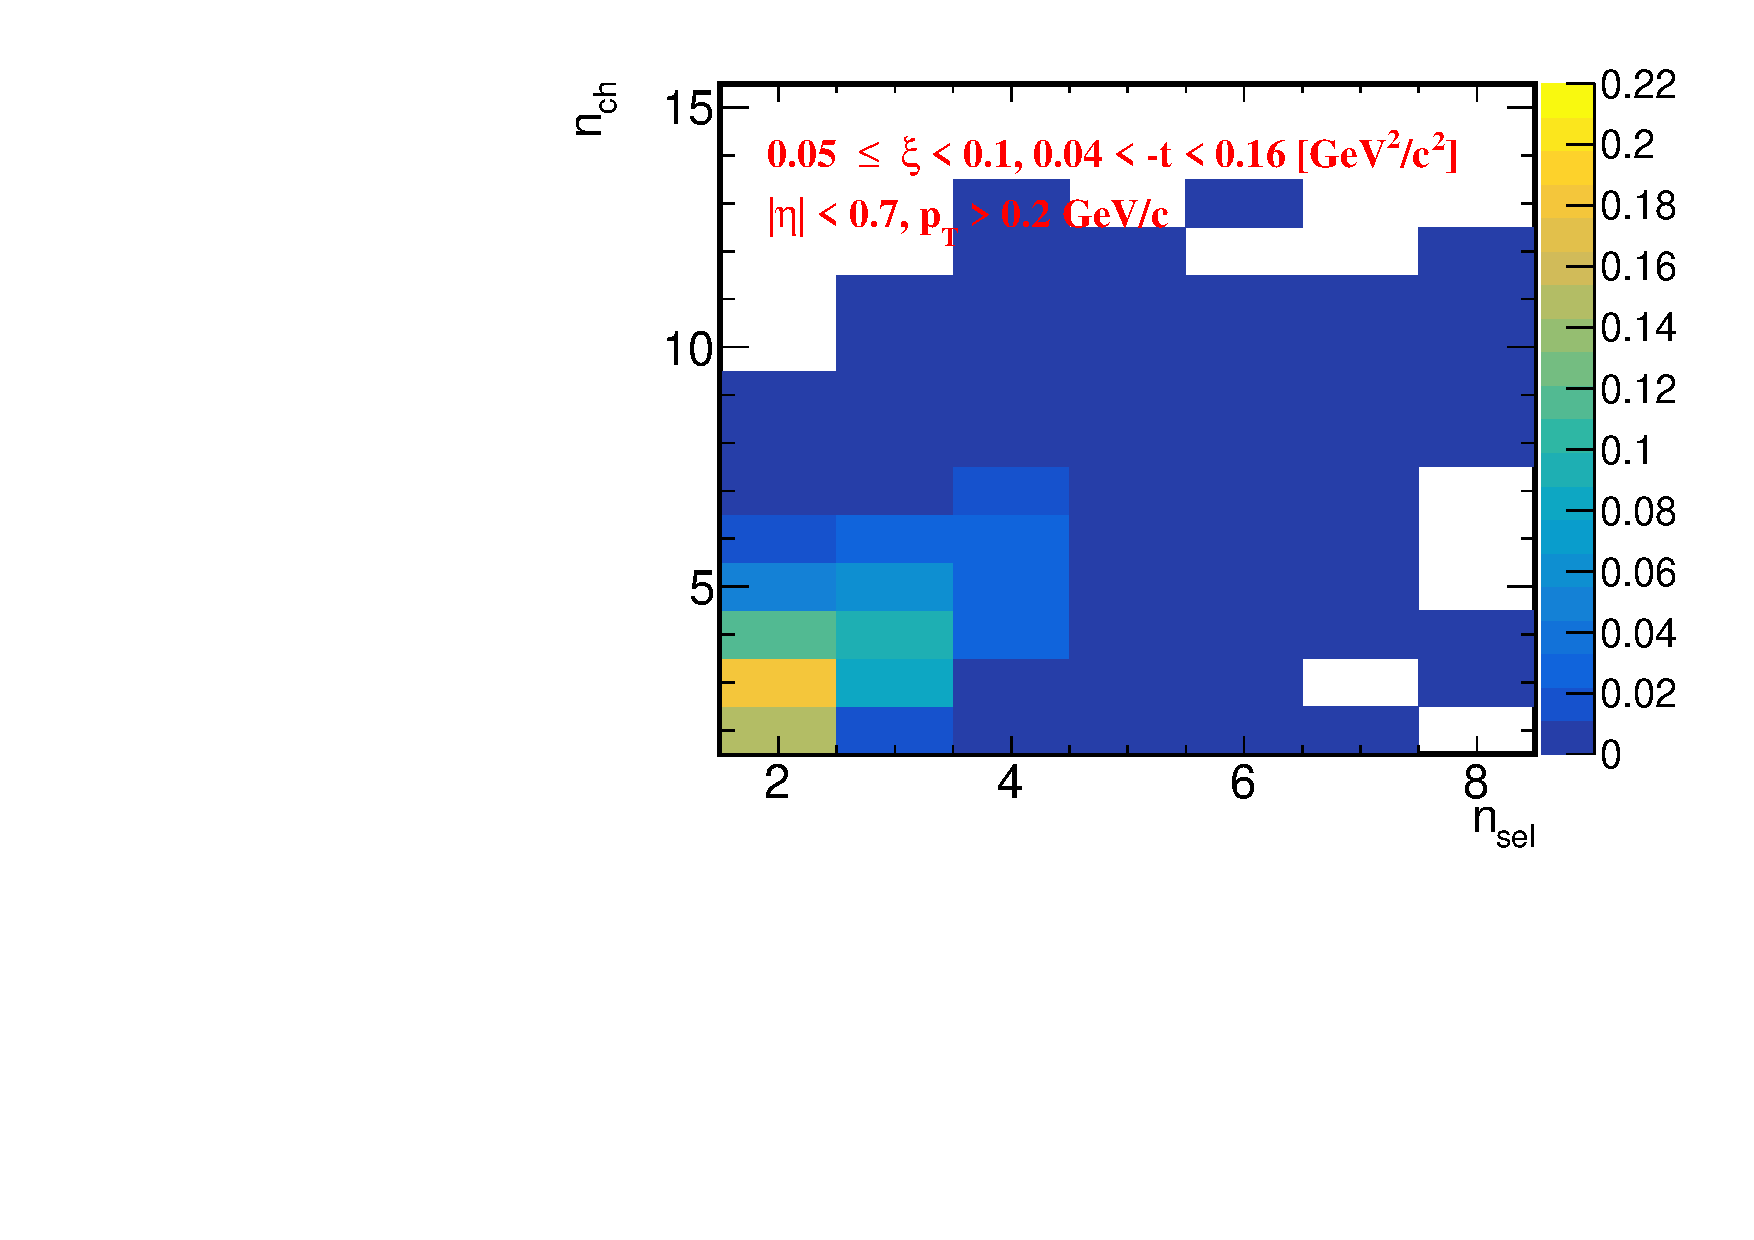
\includegraphics[width=\textwidth,page=1]{chapters/chrgSTAR/img/unfolding/matrix_1.pdf}
	\end{subfigure}
	\begin{subfigure}{.49\textwidth}
		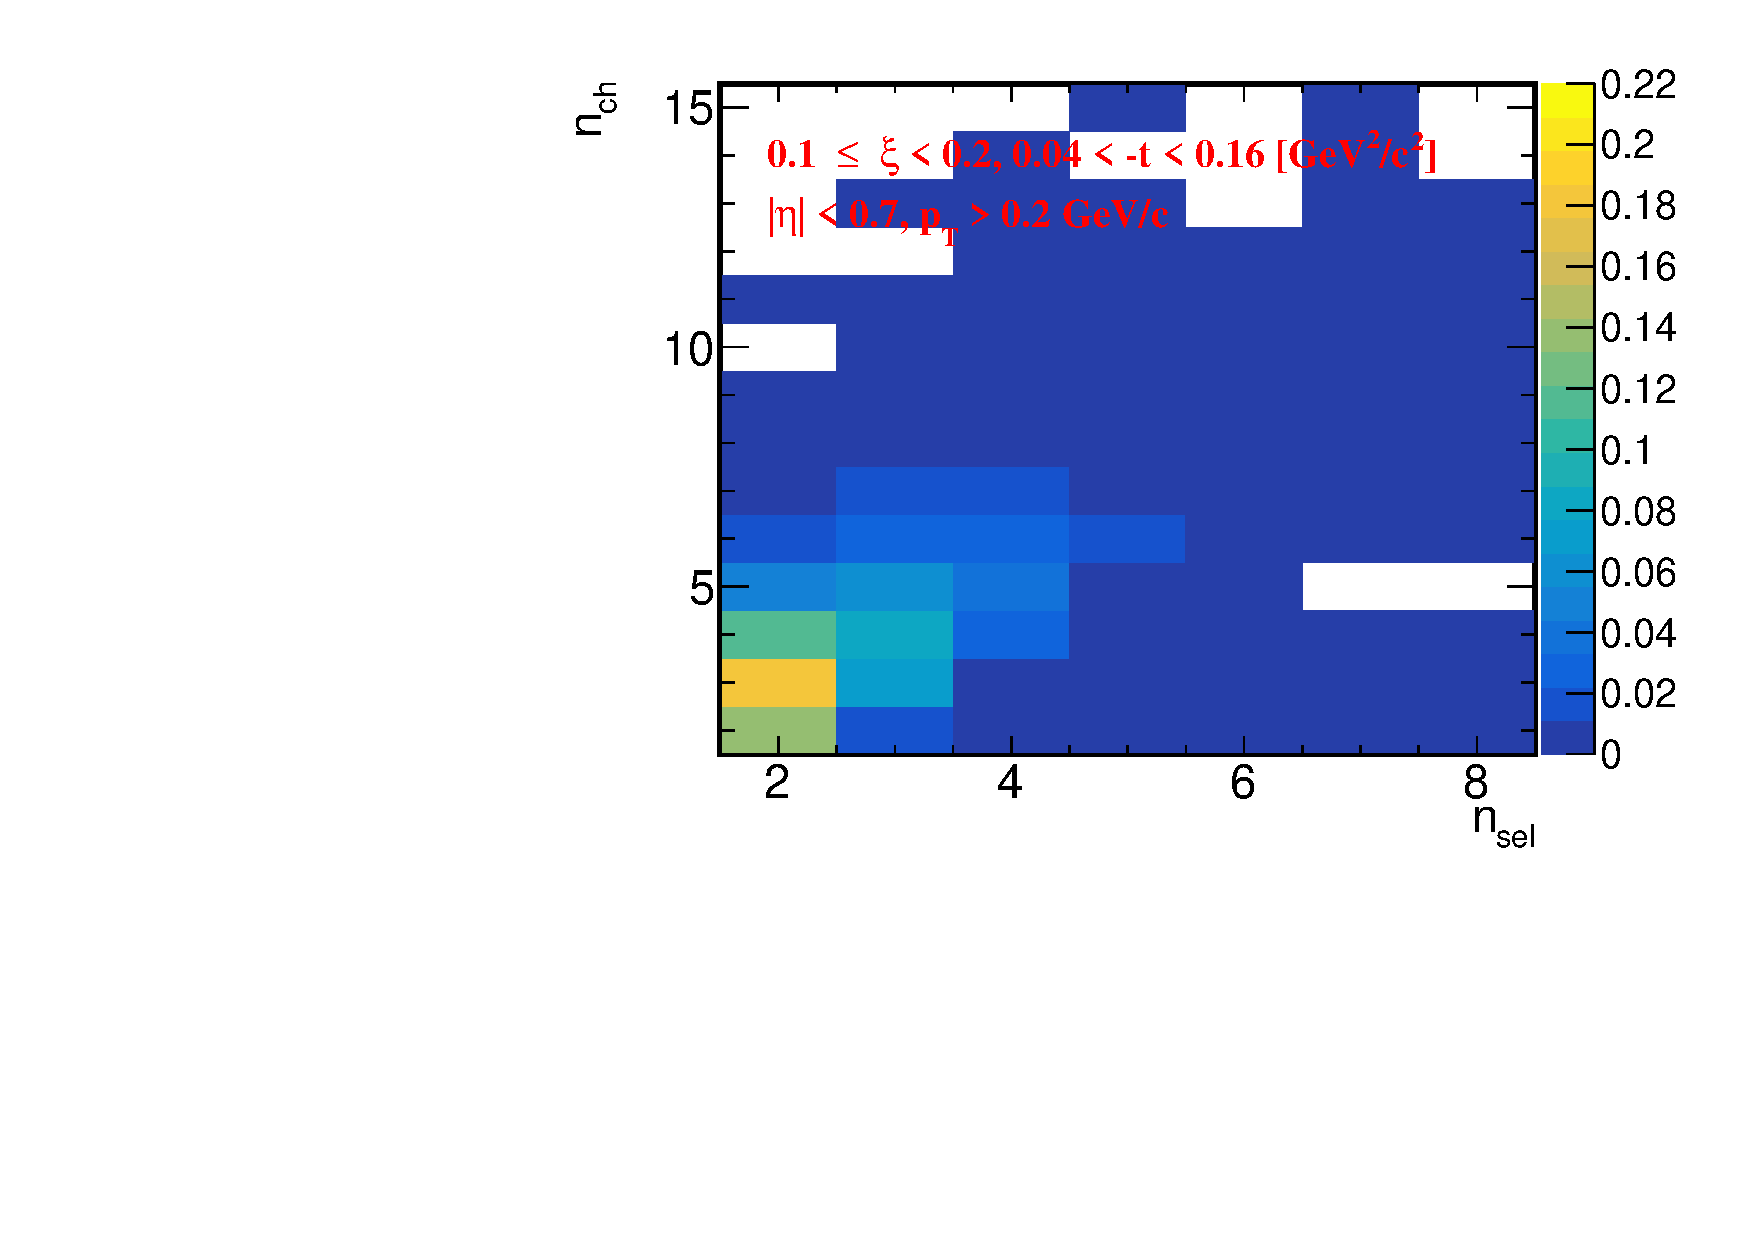
\includegraphics[width=\textwidth,page=1]{chapters/chrgSTAR/img/unfolding/matrix_2.pdf}
	\end{subfigure}
	\begin{minipage}{.49\textwidth}
		\caption{The unfolding matrices calculated  from PYTHIA~8 embedding MC for three ranges of $\xi$ separately.}
		\label{fig:responseSTAR}
	\end{minipage}
	\vspace{-0.5cm}
\end{figure}


\begin{figure}[h!]
	%\vspace{-0.5cm}
	\centering
	\begin{subfigure}{.49\textwidth}
		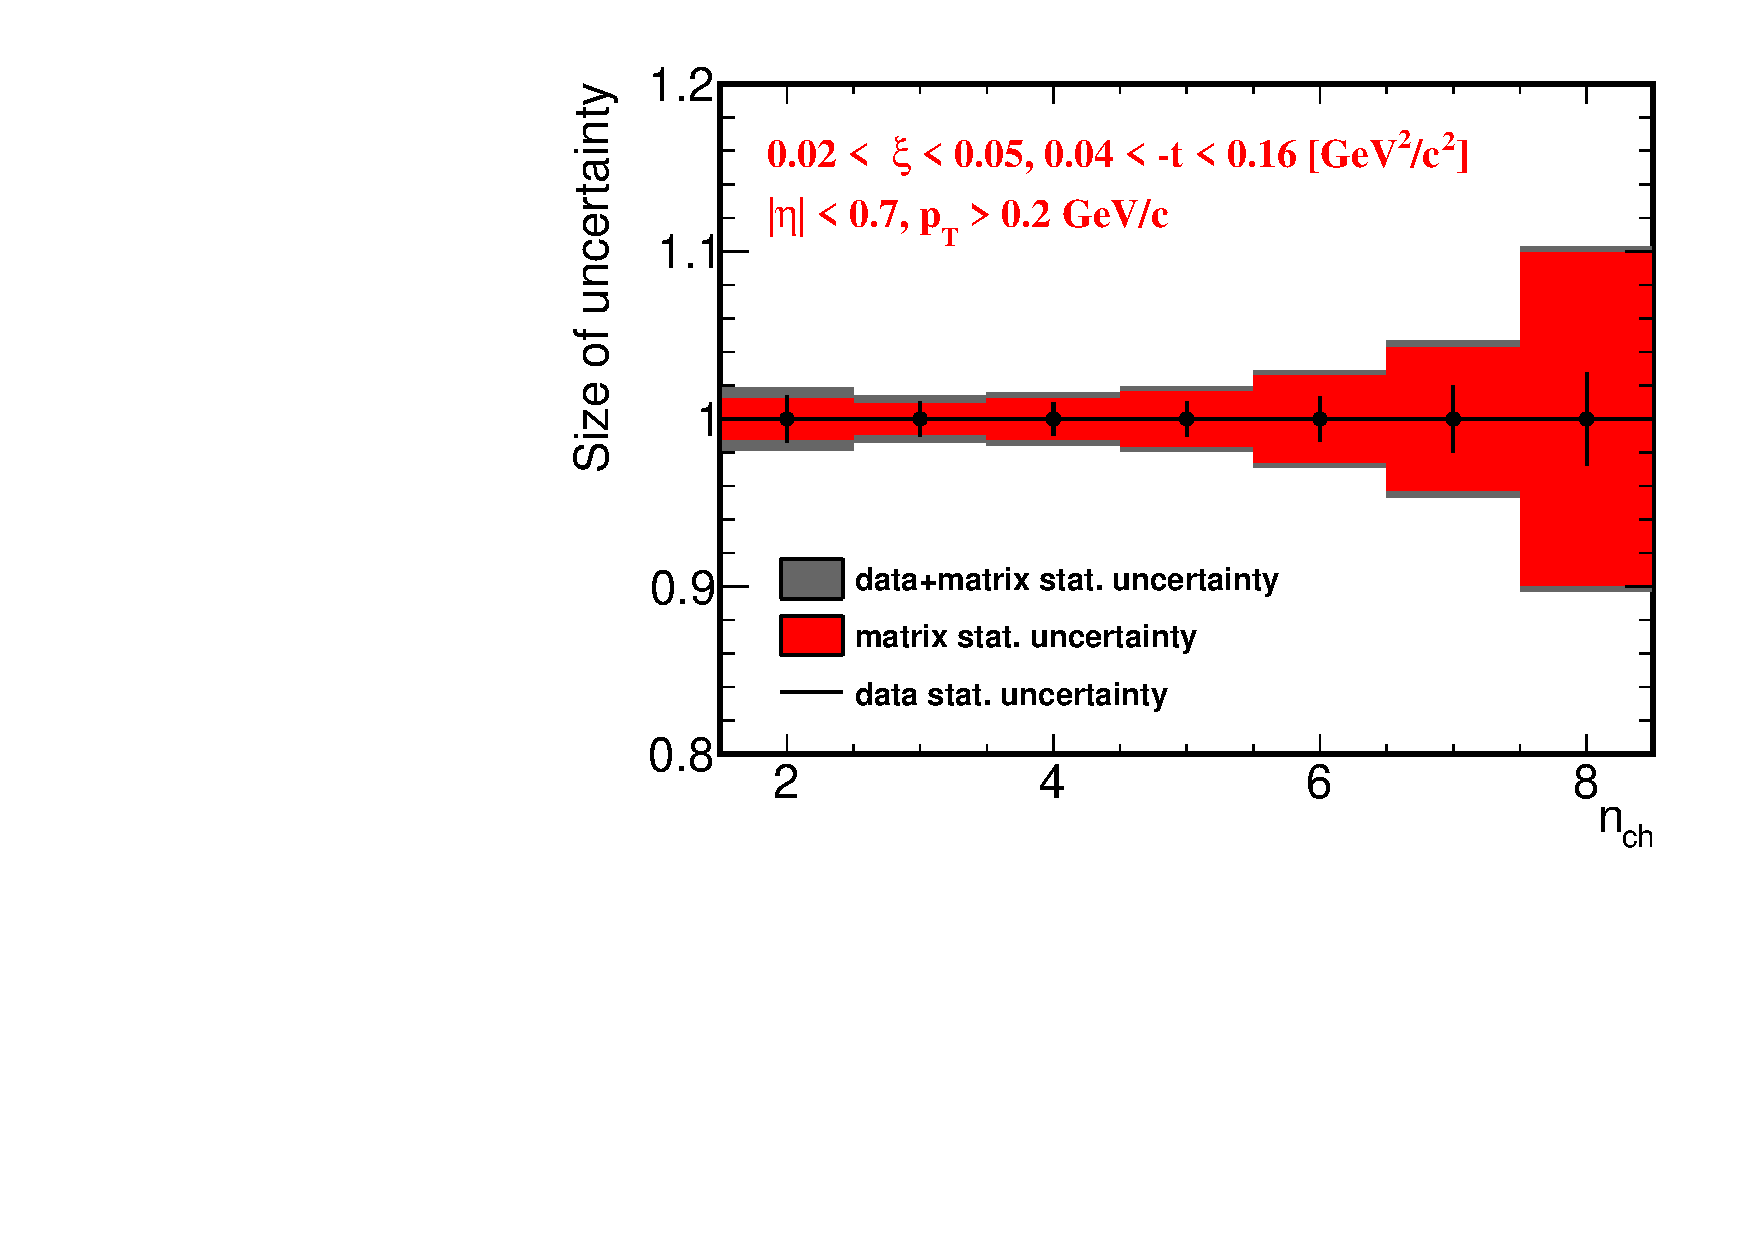
\includegraphics[width=\textwidth,page=1]{chapters/chrgSTAR/img/unfolding/matrix_stat_0.pdf}
	\end{subfigure}
	\begin{subfigure}{.49\textwidth}
		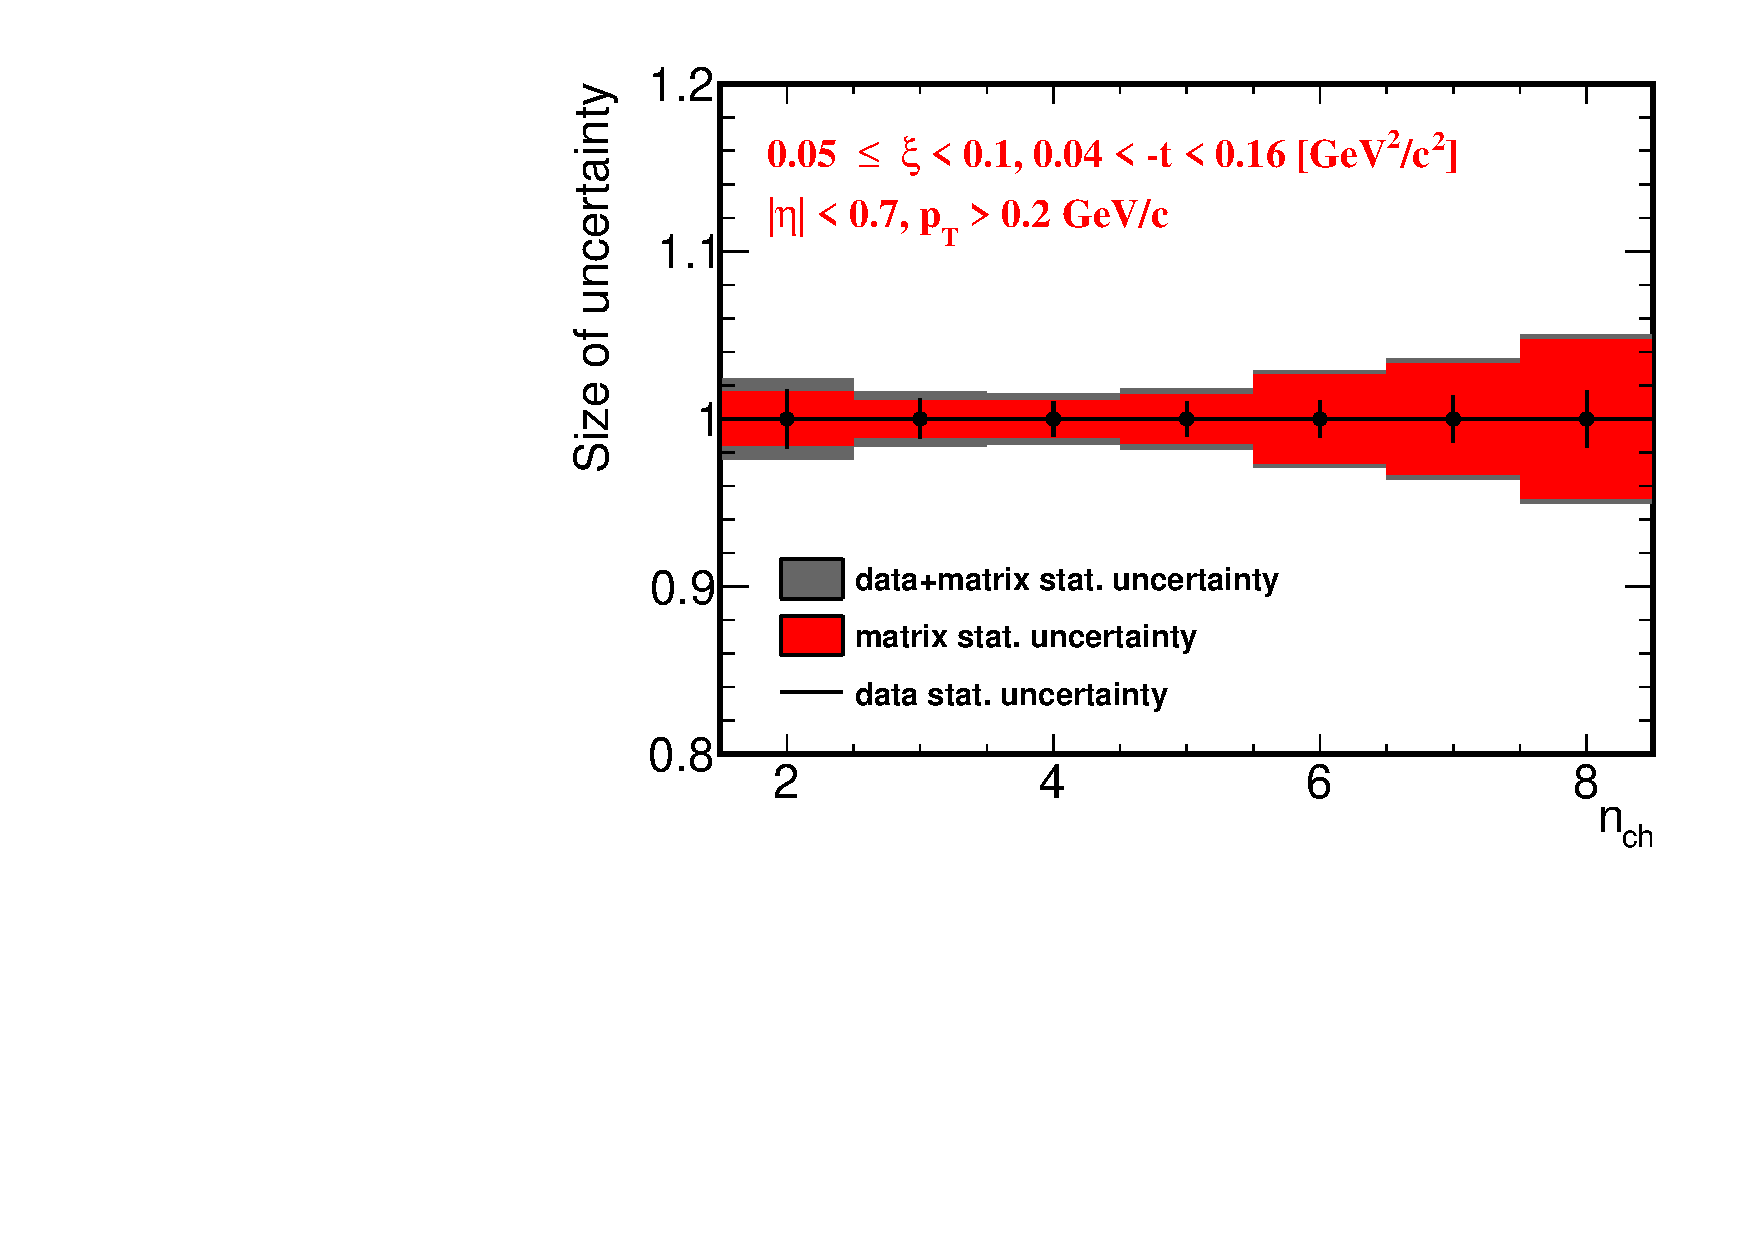
\includegraphics[width=\textwidth,page=1]{chapters/chrgSTAR/img/unfolding/matrix_stat_1.pdf}
	\end{subfigure}
	\begin{subfigure}{.49\textwidth}
		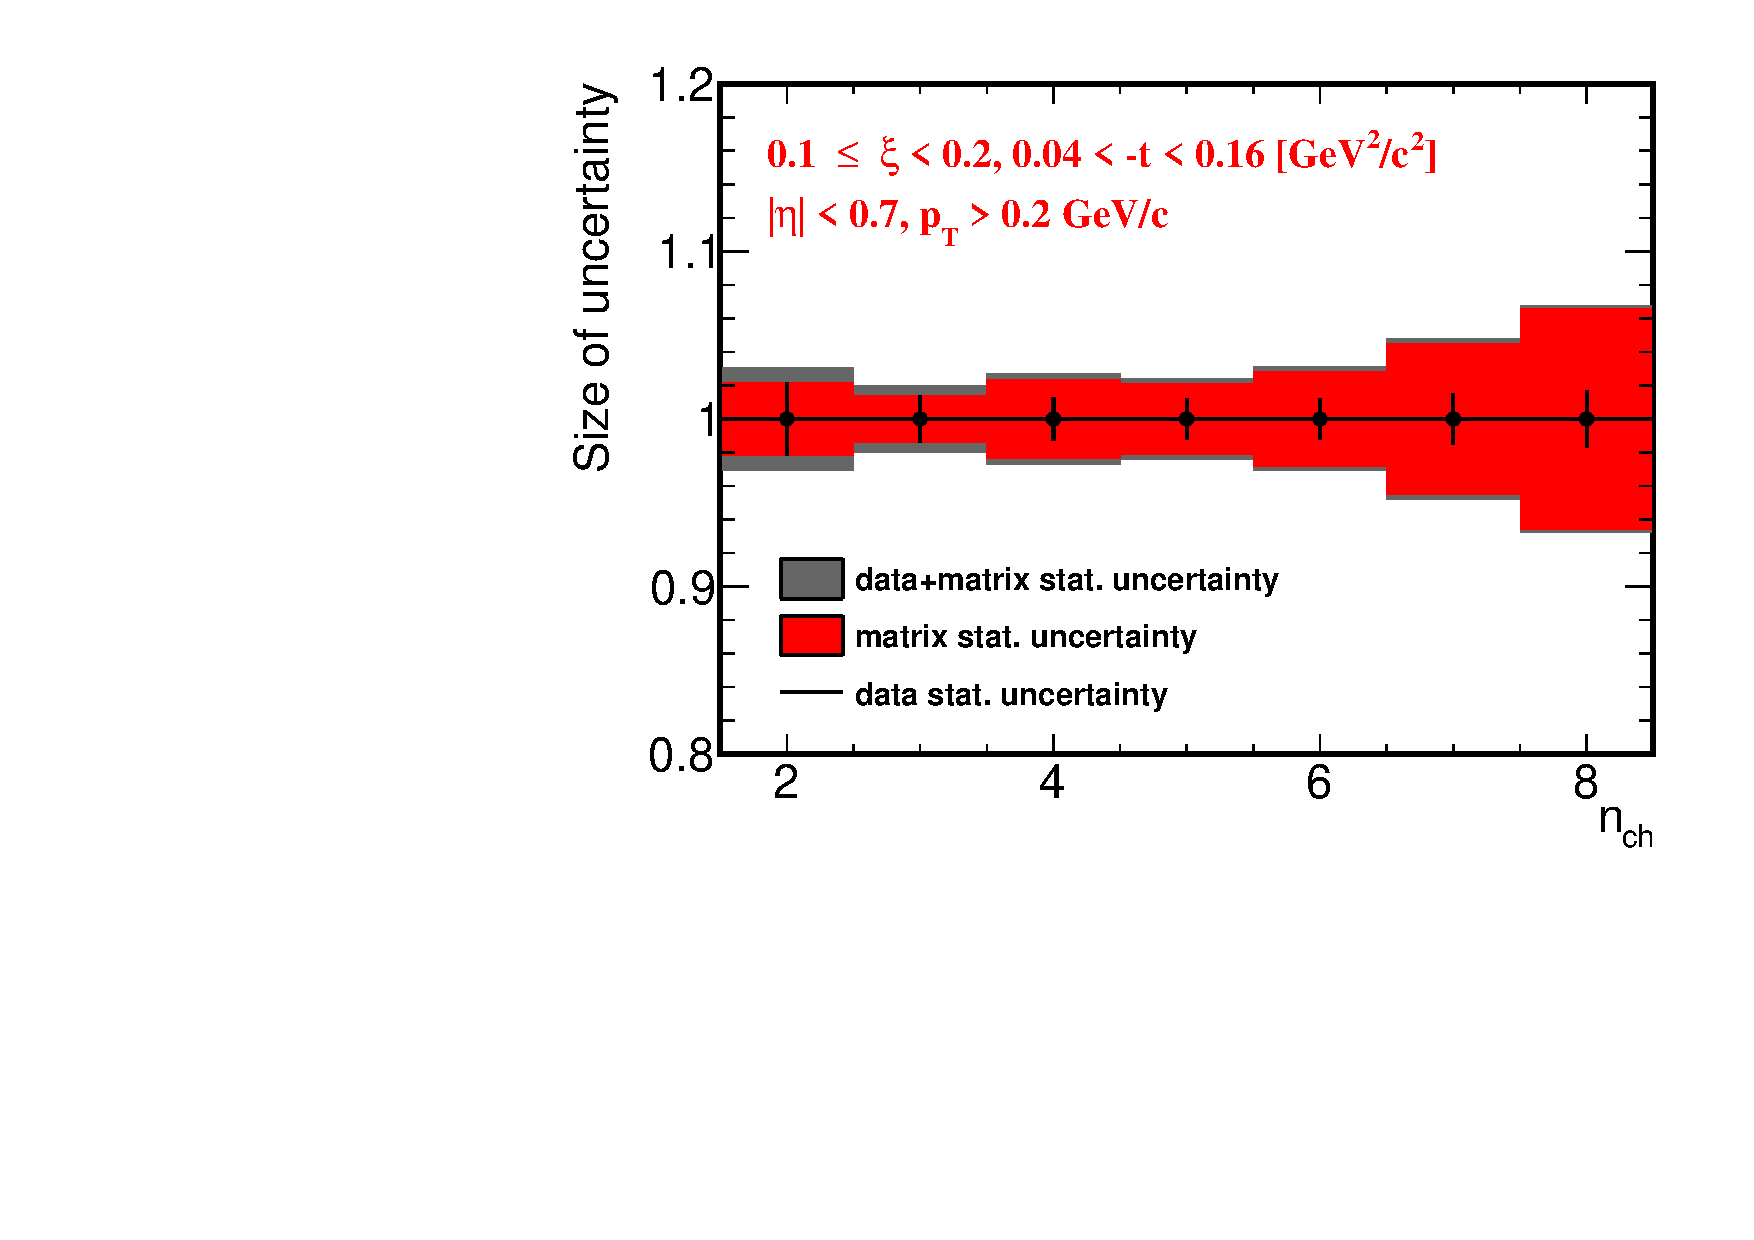
\includegraphics[width=\textwidth,page=1]{chapters/chrgSTAR/img/unfolding/matrix_stat_2.pdf}
	\end{subfigure}
	\begin{minipage}{.49\textwidth}
		\caption{Comparison of  uncertainties  related to data and PYTHIA~8 statistics  for the~charged particle multiplicity in three $\xi$ regions. 
		The~error bars represent uncertainty due to  data
		statistics. The red band shows uncertainty of the~unfolding matrices, while the gray band reflects these two added in quadrature.}
		\label{fig:responseSTAR_uncert}
	\end{minipage}
	%\vspace{-0.5cm}
\end{figure}

The distribution $dN/dn_\textrm{ch}$ obtained after the unfolding procedure
was corrected for BBC-small efficiency, through $w_\textrm{BBC}(n_\textrm{ch})$ weights, and migrations of events between $\xi$ ranges, through $f_{\xi}(n_\textrm{ch})$ weights. Since the unfolding matrices contain track reconstruction efficiencies, non-primary track backgrounds, migrations of tracks into and out of the~fiducial region, the weight $w_\textrm{trk}\left(p_\textrm{T},\eta,V_{z}\right)$ was not used.

\hspace{\parindent} Finally, the $dN/dn_\textrm{ch}$ distribution was normalized to the~total number of events, $N_\textrm{ev}=N$, which was calculated as the integral of the unfolded  distribution.



%\FloatBarrier